\documentclass[xcolor=svgnames,17pt]{beamer}

\usepackage[export]{adjustbox}
\usepackage{bookmark}
\usepackage{colortbl} \arrayrulecolor[gray]{0.7}
\usepackage{microtype}
\usepackage{pgfpages}
\usepackage{rotating}
\usepackage{textcomp}
\usepackage{tabularx}
\usepackage{xspace}
\usepackage{appendixnumberbeamer}

\usepackage{fontspec}

\hypersetup{hidelinks,pdfpagemode=}

\urlstyle{same}

\newcommand*{\sizefont}[1]{%
    \ifcase#1\relax
    \or \tiny
    \or \scriptsize
    \or \footnotesize
    \or \small
    \or \normalsize
    \or \large
    \or \Large
    \or \LARGE
    \or \huge
    \or \Huge
    \fi}

%%

\newcommand*{\mybullet}{\tikz[baseline=-.6ex]\node[%
    draw,circle,inner sep = -0.15ex,fill]{.};\xspace}

\setbeamertemplate{footline}{
    \usebeamercolor[fg]{page number in head/foot}%
    \usebeamerfont{page number in head/foot}%
    \hspace*{1ex}\insertframenumber\,/\,\inserttotalframenumber\hfill
    github.com/andrewdotn/extending-jenkins-with-jython\ }

\newcommand*{\plainfooter}{%
    \setbeamertemplate{footline}{
        \usebeamercolor[fg]{page number in head/foot}%
        \usebeamerfont{page number in head/foot}%
        \hspace*{1ex}\insertframenumber\,/\,\inserttotalframenumber\vskip2pt}}

\makeatletter
\def\alphslide{\@alph{\intcalcAdd{1}{\intcalcSub{\thepage}{\beamer@framestartpage}}}}
\newcommand*{\plainstepfooter}{
    \setbeamertemplate{footline}{
        \usebeamercolor[fg]{page number in head/foot}%
        \usebeamerfont{page number in head/foot}%
        \hspace*{1ex}\insertframenumber\alphslide\,/\,\inserttotalframenumber\vskip2pt}}
\makeatother

\setbeamertemplate{note page}{
    \sizefont{3}
    \setlength{\parskip}{10pt}
    \insertnote
    \par}

\setbeamertemplate{navigation symbols}{}
\setbeamerfont{title}{size=\LARGE}
\setbeamerfont{frametitle}{size=\LARGE}
\setbeamerfont{framesubtitle}{size=\normalsize}

\newcommand*{\tocsection}[1]{\pdfbookmark[2]{#1}{#1}}

%%

\title{Extending Jenkins \\ with Jython}

\author{\texorpdfstring{%
    Andrew Neitsch}{Andrew Neitsch}}

\date{\small 2015-10-23}

\begin{document}

\tocsection{Title page}

\begin{frame}[plain]
\titlepage
\adjustbox{width=0.9\paperwidth,center}{\structure{\href{https://github.com/andrewdotn/extending-jenkins-with-jython}{github.com/andrewdotn/extending-jenkins-with-jython}}}
\end{frame}

\note{This is a note}

\begin{frame}{Outline}
\tableofcontents
\end{frame}

\section{Introduction}

\begin{frame}{Jenkins}

\begin{itemize}
\item Industry-standard continuous integration tool
\item Regularly and automatically builds and tests your code
\item Helps make sure your code works, and stays working
\end{itemize}

\end{frame}

\begin{frame}{Example: Testing hello}
% TODO: screenshot
\end{frame}

\begin{frame}{}
If you have tests, you’re already running them before you commit, so why
bother?
\pause
\begin{itemize}
\item Can test regularly forever, not just when there’s a change
\pause
\item Multi-configuration builds: different Python versions, library
versions, platforms, Linux, Windows, and Mac
\end{itemize}
\pause
\alert{These are really valuable things that nobody will consistently do by
hand!}
\end{frame}

\begin{frame}{Example: hello v2, using six}

\end{frame}

\begin{frame}{Advanced uses}

\begin{columns}
\column{.4\textwidth}
\fbox{%
    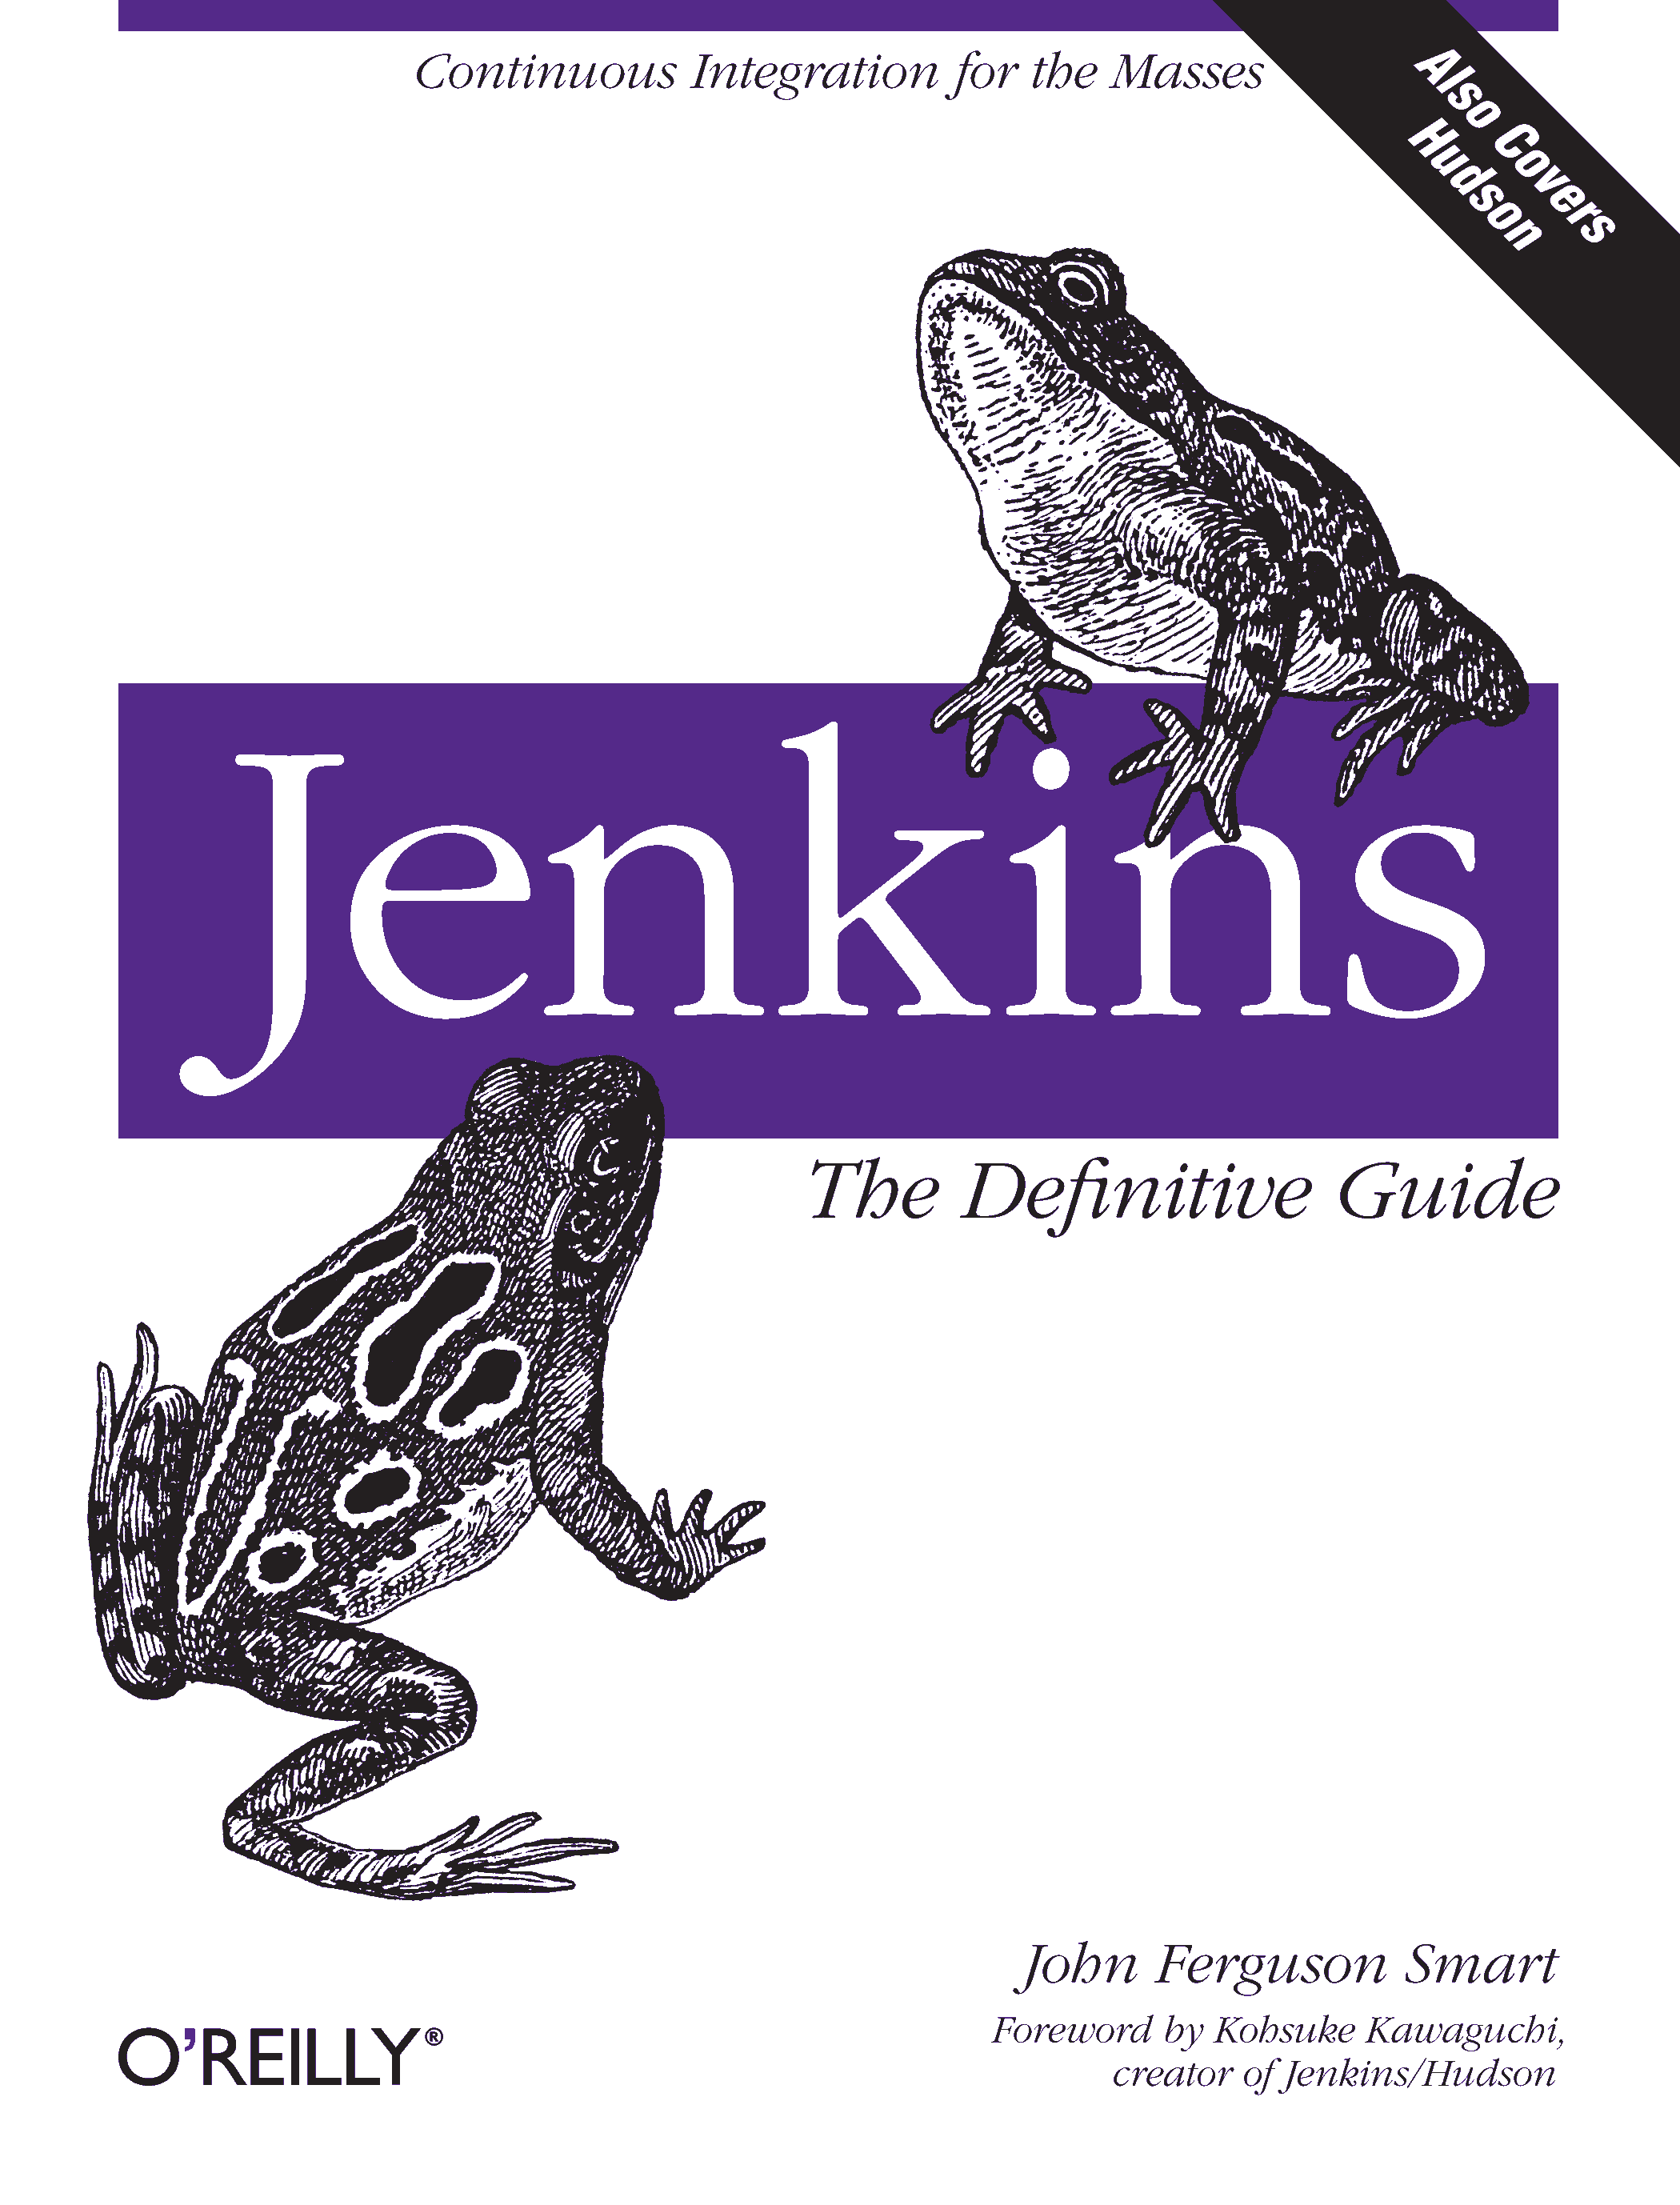
\includegraphics[width=\textwidth]{jenkins-the-definitive-guide.png}}
\column{.6\textwidth}
\begin{itemize}
\item Try servers
\item Track betas and release candidates
\item Automated deployments
\end{itemize}
\end{columns}

\end{frame}

\section{Test Isolation}

\begin{frame}{}
\tableofcontents[currentsection]
\end{frame}

\begin{frame}[plain]{}

\includegraphics[height=0.95\paperheight,center]{works-on-my-machine.pdf}
\end{frame}

\begin{frame}[plain]{}

\includegraphics[height=0.95\paperheight,center]{works-on-jenkins.pdf}
\end{frame}

\begin{frame}{}

\includegraphics[width=0.95\paperwidth,center]{docker-logo.pdf}
\begin{center}
Project goal: %
\href{https://blog.docker.com/2014/10/docker-microsoft-partner-distributed-applications/}{%
“To build the ‘button’ that enables any application to be built and
deployed on any server, anywhere.”}
\end{center}
\end{frame}

\begin{frame}{Testing using docker}
\end{frame}

\begin{frame}{More examples}
\begin{itemize}
\item \href{https://stripe.com/blog/distributed-ruby-testing}{%
    \structure{Running three hours of Ruby tests in under three minutes}}
\end{itemize}
\pause
Maybe someone will give a talk on useful things Docker can do for Python
developers?
\end{frame}

\section{Extending Jenkins}

\begin{frame}[plain]{}
\tableofcontents[currentsection]
\end{frame}

\begin{frame}[plain]{}
\begin{columns}
\column{.4\textwidth}
Jenkins is extremely extensible \\
\vspace*{\baselineskip}
1,000+ plugins(!)
\column{.6\textwidth}
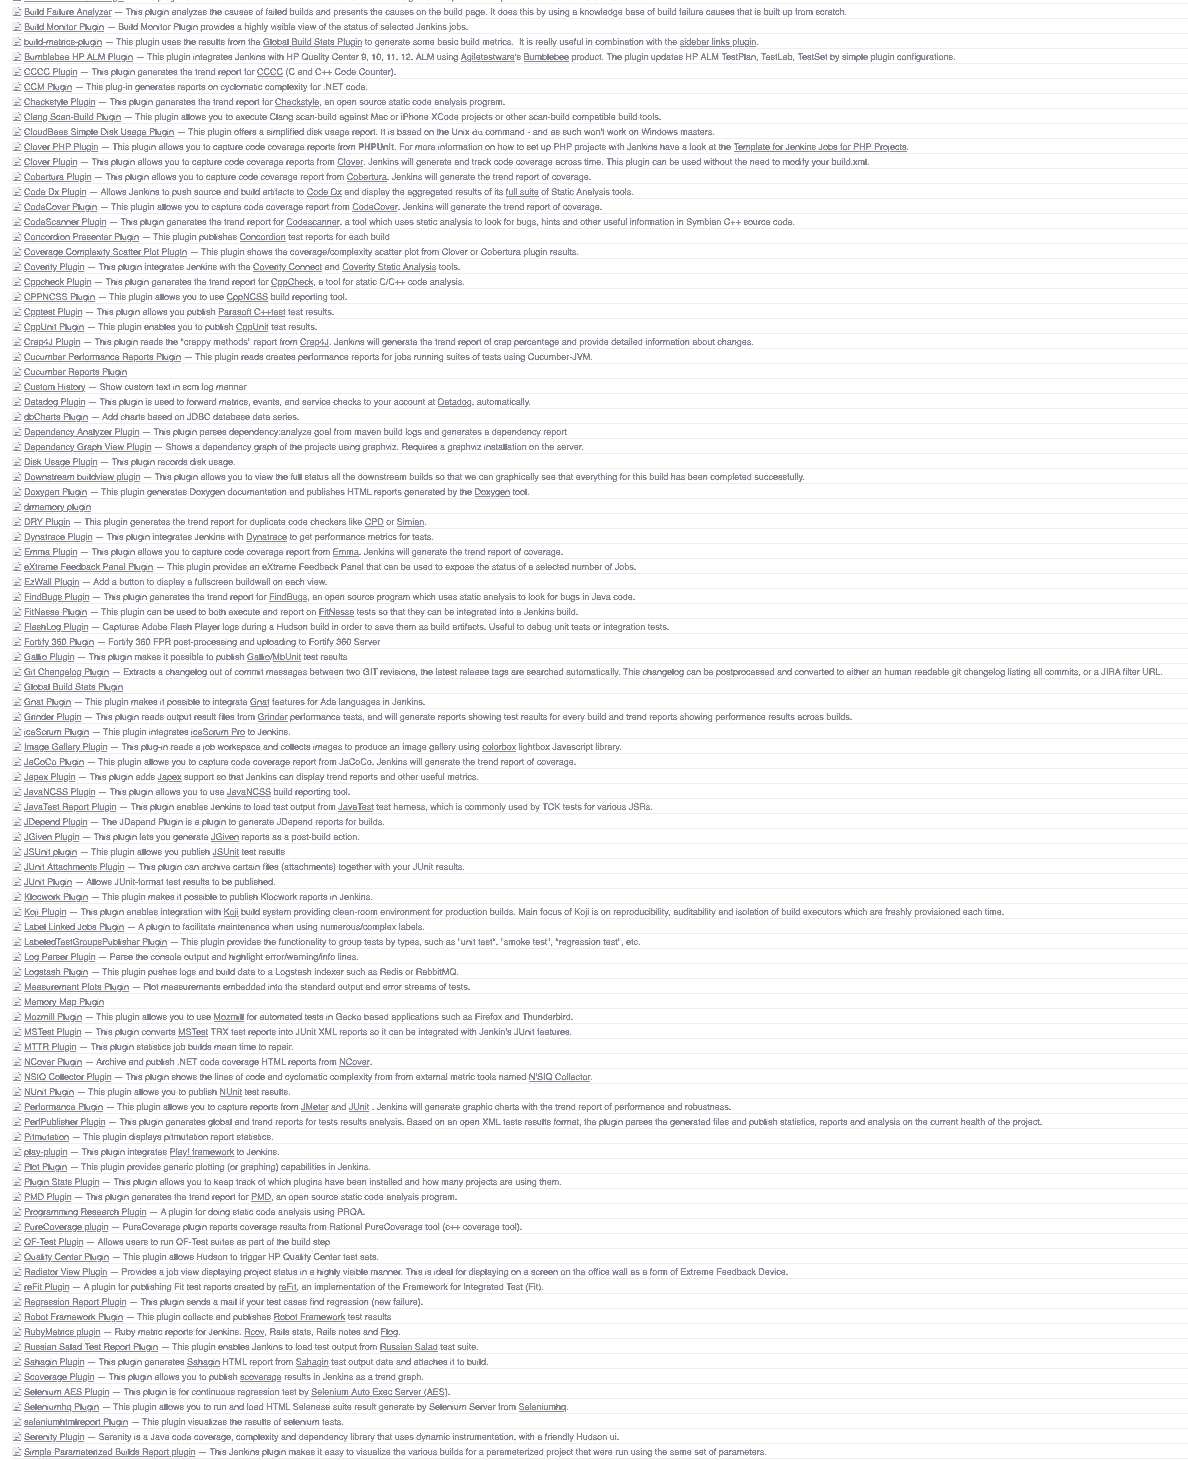
\includegraphics[height=\paperheight]{plugin-list.png}
\end{columns}
\end{frame}

\begin{frame}{Use case: Code metrics}
Would be nice to see things like
\begin{itemize}
\item Code coverage rates
\item Function documentation rates
\item Style compliance rates
\item Lines of code
\item Number of slides in presentation
\end{itemize}
All right on the dashboard
\end{frame}

\begin{frame}{Jenkins is written in Java}

\pause
\begin{center}
What about Jython?
\end{center}

\end{frame}

\begin{frame}{Issues}
\begin{itemize}
\item Compile-time annotations and extension discovery
\pause
\item Jython scripts can call Java  much more easily than Java can call
Jython
\only<2>{
\end{itemize}
\sizefont{2}\texttt{%
PythonInterpreter interpreter = new PythonInterpreter(); \\
interpreter.exec("from Building import Building"); \\
buildingClass = interpreter.get("Building"); \\
PyObject buildingObject = buildingClass.\_\_call\_\_( \\
\ \ \ \ new PyString(name), PyString(location), \\
\ \ \ \ new PyString(id)); \\
return (BuildingType)buildingObject \\
\ \ \ \ .\_\_tojava\_\_(BuildingType.class);}
\begin{itemize}
}
\pause
\item Newer tool \href{https://github.com/jythontools/clamp}{\structure{clamp}},
can only invoke interface methods
\end{itemize}
\end{frame}

\begin{frame}{Success}
PythonWrapper and
\href{https://github.com/jenkinsci/jenkins.py/tree/master/ppsm}{\structure{ppsm}}

\vspace*{\baselineskip}

\pause

Really well done!

\vspace*{\baselineskip}

\pause

Main development technique:
\begin{itemize}
\item View source for existing plugins
\item And Jenkins source code
\end{itemize}
\end{frame}


\begin{frame}[fragile]{Working example}

See the \texttt{jython-hello-world} directory.

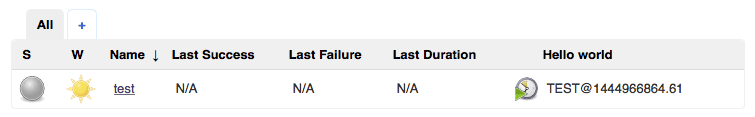
\includegraphics[width=\textwidth]{jython-hello-world.png}

\vspace*{-0.5\baselineskip}

{\sizefont{1}
\begin{verbatim}
def hello(job):
    return job.getName().upper() + "@" + str(time.time())
...
<j:jelly xmlns:j="jelly:core">
  <td>${it.hello(job)}</td>
</j:jelly>
...
@Extension
public class HelloWorldColumn extends ListViewColumnPW {
    public String hello(Object o) {
        return execPython("hello", o).toString();
    }
}
\end{verbatim}
}

\end{frame}

\begin{frame}{Still need to learn guts}
\begin{itemize}
\item Jelly XML-based template/data-binding language
\item Java data model
\end{itemize}
\pause

\begin{center}
Writing a whole plugin in Python \\ doesn’t feel like a net win \\
\pause
but calling a Python library \\ from Java definitely could be
\end{center}

\end{frame}

\section{Conclusions}

\begin{frame}{}
\tableofcontents[currentsection]
\end{frame}

\begin{frame}{Conclusions}
\begin{itemize}
\item Jenkins runs tests that humans don’t have the patience to run by
hand: multiple Python versions, multiple platforms, every commit, every day
\pause
\item You can help your fellow developers by making tests that will run
anywhere
\pause
\item You can extend Jenkins with Jython ...
\pause but there will still be a lot of Java.
\end{itemize}
\end{frame}

\appendix

\begin{frame}
\adjustbox{width=0.5\paperwidth,center}{\structure{Questions?}}
\end{frame}

\begin{frame}{Call for talks}

“w/o interesting talks, there's not a ton of point in ‘meeting up’”

\pause

\begin{enumerate}
\item Pick something you find interesting
\item Talk about it
\item Include exercises for people to hack on
\end{enumerate}

\end{frame}

\begin{frame}{Suggested exercises}
\begin{itemize}
\item Install Jenkins, and get it testing \\ some code you care about
\item Isolate your tests
\item Try extending Jenkins
\end{itemize}
\end{frame}

\end{document}
